\documentclass[12pt]{article}

\usepackage[a4paper,margin=2.5cm]{geometry}
\usepackage{amsmath, amssymb, amsthm}
\usepackage{bm}
\usepackage{hyperref}
\usepackage{graphicx}
\usepackage{caption}
\usepackage{listings}
\usepackage{xcolor}
\usepackage{float}
\usepackage{placeins}
\graphicspath{{figures/}}

\lstdefinestyle{code}{
  basicstyle=\ttfamily\small,
  numbers=left,
  numberstyle=\tiny,
  numbersep=8pt,
  keywordstyle=\color{blue},
  commentstyle=\color{teal!70!black},
  stringstyle=\color{orange!70!black},
  showstringspaces=false,
  breaklines=true,
  frame=single,
  framerule=0.3pt,
  rulecolor=\color{black!15}
}
\lstset{style=code}

\title{Advantage Actor-Critic (A2C) Tutorial}
\author{}
\date{\today}

\begin{document}
\maketitle

\section{Introduction}
Advantage Actor-Critic (A2C) is a synchronous variant of the actor-critic framework where a policy (actor) is updated using gradients weighted by advantage estimates supplied by a value function (critic). By updating both components jointly, A2C stabilizes policy gradient learning and supports synchronous batching across environments.

\section{Theory and Formulas}
\subsection{Actor-Critic Objective}
With policy \(\pi_\theta(a\mid s)\) and value function \(V_w(s)\), the policy gradient uses the advantage function \(A^{\pi}(s,a) = Q^{\pi}(s,a) - V^{\pi}(s)\):
\begin{equation}
\nabla_\theta J(\theta) = \mathbb{E}_{s,a}\big[ \nabla_\theta \log \pi_\theta(a\mid s)\, A^{\pi}(s,a) \big].
\end{equation}
Temporal-difference (TD) error provides a low-variance estimate of the advantage.

\subsection{Critic Update}
The critic minimizes the squared TD error
\begin{equation}
\delta_t = r_{t+1} + \gamma V_w(s_{t+1}) - V_w(s_t), \qquad w \leftarrow w + \beta \delta_t \nabla_w V_w(s_t).
\end{equation}
In tabular settings \(V_w\) is simply updated with \(V(s_t) \leftarrow V(s_t) + \beta \delta_t\).

\subsection{Actor Update}
The actor performs gradient ascent using the same TD error as an advantage estimate:
\begin{equation}
\theta \leftarrow \theta + \alpha \delta_t \nabla_\theta \log \pi_\theta(a_t\mid s_t).
\end{equation}
Entropy regularization \(H[\pi_\theta(\cdot\mid s)]\) is often added to encourage exploration. A2C typically executes multiple environments in parallel, synchronizes gradients, and updates parameters in a single batch.

\section{Applications and Tips}
\begin{itemize}
  \item \textbf{Discrete control}: grid-world navigation, Atari benchmarks with synchronous rollouts.
  \item \textbf{Multi-environment training}: leverage vectorized simulators to reduce variance.
  \item \textbf{Low-latency robotics}: when on-policy updates are feasible and stability is needed.
  \item \textbf{Best practices}: normalize advantages, tune entropy coefficients, monitor actor and critic losses separately, and ensure value targets remain in range via gradient clipping.
\end{itemize}

\section{Python Practice}
The script \texttt{gen\_a2c\_figures.py} trains a tabular A2C agent on a grid-world with terminal rewards. It visualizes the learning curve and the critic's value estimates after training.
\begin{lstlisting}[language=Python,caption={Excerpt from gen_a2c_figures.py}]
prob = softmax(theta[state])
action = rng.choice(n_actions, p=prob)
next_state, reward, done = env.step(state, action)
td_error = reward + gamma * V[next_state] * (1.0 - float(done)) - V[state]
V[state] += critic_lr * td_error
theta[state] += actor_lr * td_error * (one_hot(action, n_actions) - prob)
\end{lstlisting}

\section{Result}
\begin{figure}[H]
  \centering
  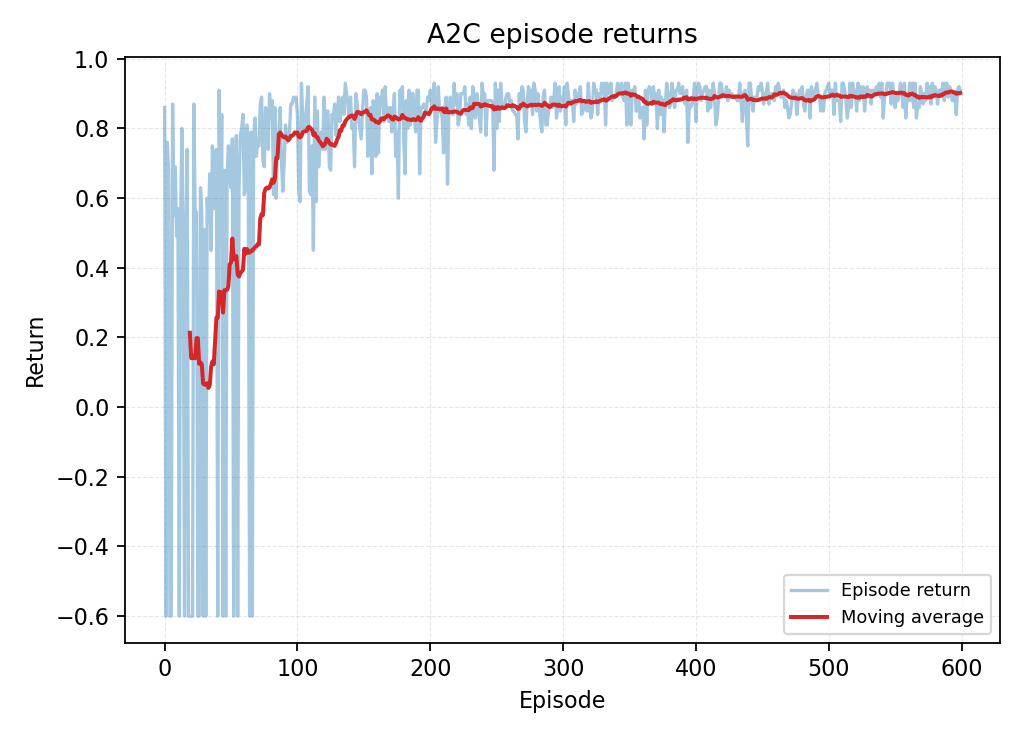
\includegraphics[width=0.8\linewidth]{a2c_returns.png}
  \caption{Episode returns during A2C training with moving average smoothing}
  \label{fig:a2c_returns}
\end{figure}

\begin{figure}[H]
  \centering
  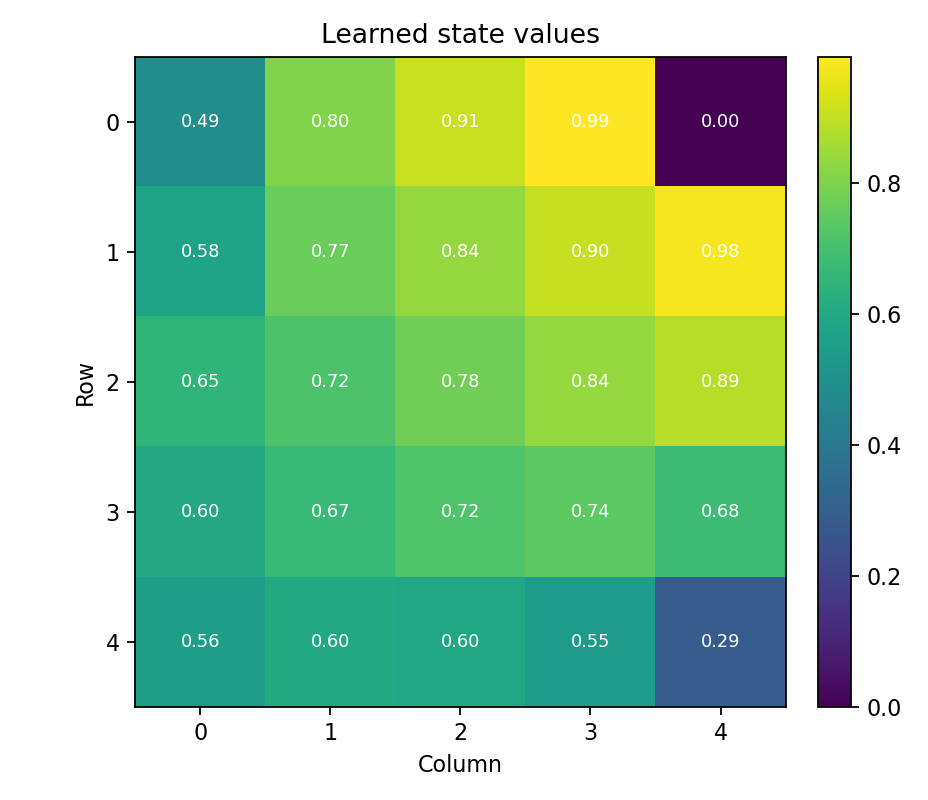
\includegraphics[width=0.82\linewidth]{a2c_value_baseline.png}
  \caption{Value function heatmap learned by the critic, highlighting preferred routes}
  \label{fig:a2c_value_baseline}
\end{figure}

\FloatBarrier
\section{Summary}
A2C synchronously updates actor and critic to reduce variance and stabilize policy gradients. Proper batching, advantage normalization, and entropy control ensure robust performance. The grid-world example demonstrates steadily improving returns and interpretable value estimates that capture the shortest-path structure.

\end{document}